% !TEX encoding = UTF-8 Unicode

\documentclass[aspectratio=169]{beamer}
\usepackage[utf8]{inputenc}

%% BIB
\usepackage[
  style=authoryear,
  backend=biber,
  url=false,
  maxcitenames=2,
  uniquename=false,
  uniquelist=false
]{biblatex}
%\addbibresource{?.bib}

%% GRAPHICS

\usepackage{graphicx}
\graphicspath{{images/},{figures/}}
\usepackage{tikz}

%% COLORS
\definecolor{UWRed}{HTML}{C5050C}
\definecolor{TintedBG}{HTML}{EEEEFF}
%\definecolor{StrongBlue}{HTML}{3F8FD2}
%\definecolor{StrongGreen}{HTML}{36C88E}
%\definecolor{StrongRed}{HTML}{9B0000}
%\definecolor{MyC}{HTML}{009999}
%\definecolor{MyM}{HTML}{990099}
%\definecolor{MyY}{HTML}{999900}
%\definecolor{MyR}{HTML}{990000}
%\definecolor{MyG}{HTML}{009900}
%\definecolor{MyB}{HTML}{000099}
%\definecolor{ActionRed}{HTML}{990000}

%% SLIDE COLOR SETTINGS
\setbeamercolor{structure}{fg=UWRed}
\setbeamercolor{title page}{fg=white}
\setbeamercolor{title}{fg=white}

%% RM NAV SYMBOLS
\setbeamertemplate{navigation symbols}{}

%% FONTS
\setbeamerfont{title}{size=\huge\bfseries}

%% DRAWING
%\usetikzlibrary{}

\def\firstcircle{(90:0.3cm) circle (0.6cm)}
\def\secondcircle{(210:0.3cm) circle (0.6cm)}
\def\thirdcircle{(330:0.3cm) circle (0.6cm)}

%% LOGO on slides
\logo{\begin{tikzpicture}[overlay]
  \node[anchor=north east,inner sep=0] at (0,86mm) {
\includegraphics[height=10mm]{SMPH_color-flush.pdf}};
\end{tikzpicture}}

%% CONTENT BEGINS

\title{Anchors (and other) High-Precision Model-Agnostic Explanations}
\subtitle{AIRG Presentation}
\author{Yuriy Sverchkov}
\institute{University of Wisconsin--Madison}
\date{October 31, 2018}

\begin{document}

  {
    \setbeamertemplate{background canvas}{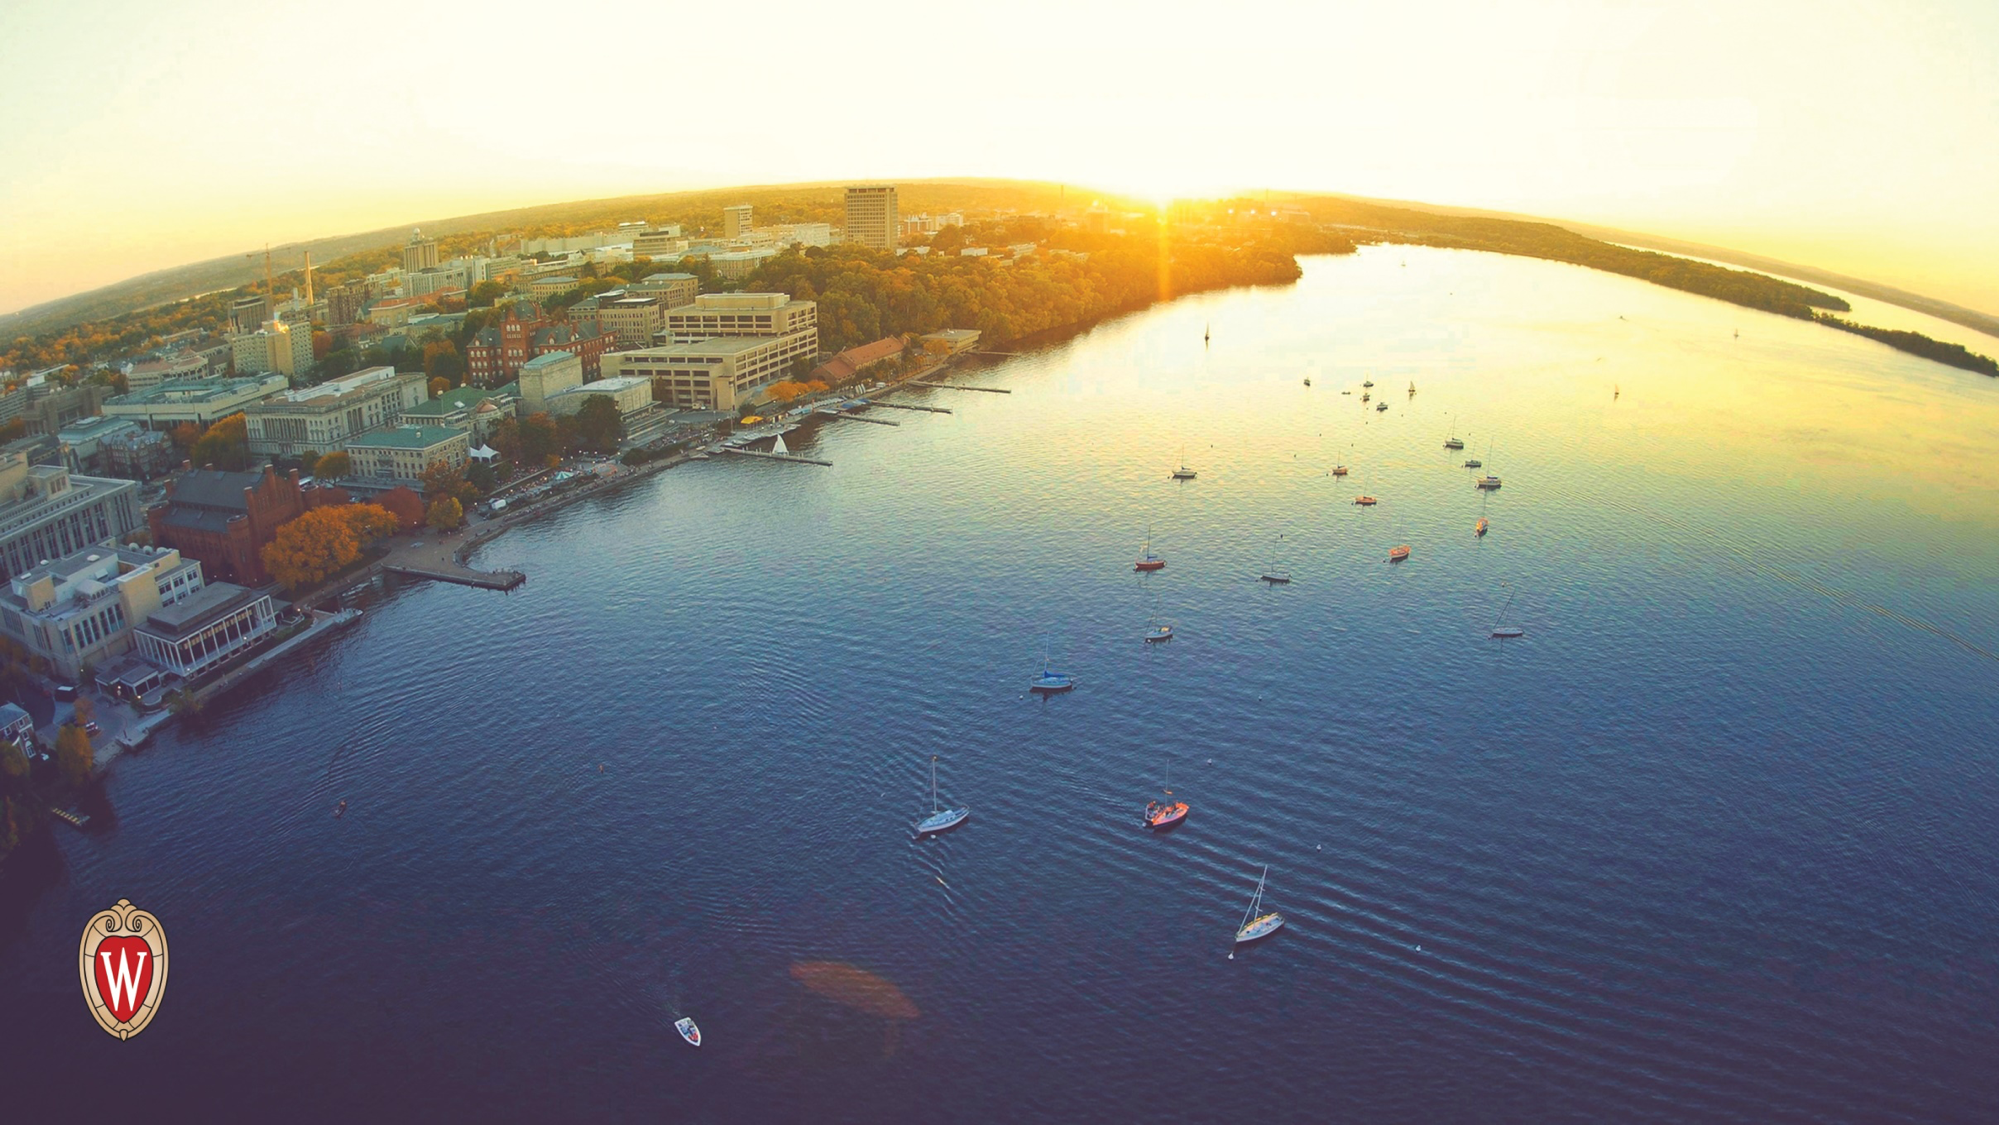
\includegraphics[width=\paperwidth]{UW-lake.png}}
    \begin{frame}[plain]
      \vskip4cm
      \titlepage
    \end{frame}
  }

%%% FRAMEBREAK %%%

% Motivation:
%  (many good ml systems are black box)
%  "chat vignette": what dis? cat! why? math! *confused* ; better explanation
%
%  (there is a need from)
%  policymakers/legal: GDPR (find the ref)
%  high-risk decision-makers: (doctors/critical systems/self-driving)
%  explanations build trust (find a ref?)

\begin{frame}{\textbf{Why} should we \textbf{explain} our models?}

\begin{itemize}[<+->]
	\item Many of the best-performing machine learning models are not (easily) \textbf{interpretable} (by non-ML experts)
	\item Users need explanations:
	\begin{itemize}
		\item when using models for medical decisions
		\item when using models for policymaking
		\item in other high-risk decision support
		\item for legal reasons
	\end{itemize}
\end{itemize}
\pause

\textbf{GDPR Article 13(2f)} [The data subject shall be informed of] the existence of automated decision-making [... and provided] meaningful information about the logic involved

\begin{itemize}[<+->]
	\item Explanations build trust in a good model
	\item Explanations can help troubleshoot a bad model
\end{itemize}
\end{frame}

%%% FRAMEBREAK %%%

\begin{frame}{Troubleshooting a model at a glance}
\vfill

\centering
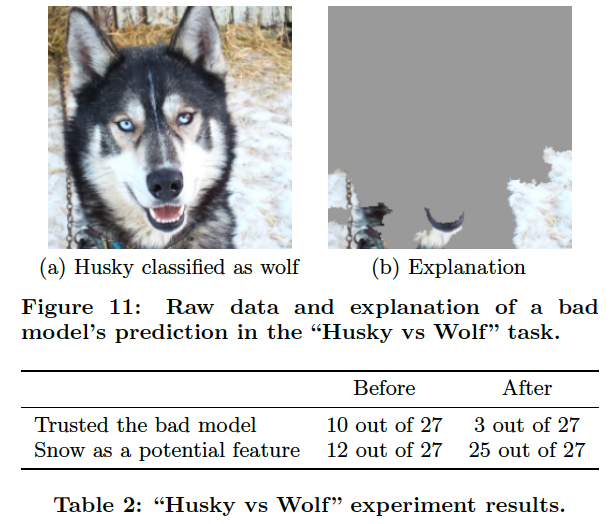
\includegraphics[width=6cm]{LIME-wolf.png}

\vfill

\raggedleft
\scriptsize
Ribiero, Singh, and Guestrin, SIGKDD 2016
\end{frame}

%%% FRAMEBREAK %%%

\begin{frame}{Interpretable models}
\begin{columns}
	\column[T]{0.45\textwidth}
	\begin{center}\bf Interpretable \end{center} \pause
	\begin{itemize}
		\item Generalized linear models
		\item[] $y = g^{-1}( X\beta )$ \pause
		\item[] For each feature $i$, $\beta_i$ tells us about its contribution:
		\begin{itemize}
			\item sign (e.g. increase vs. decrease of a risk due to a factor)
			\item magnitude (relative importance of features)
		\end{itemize} \pause
		\item Rules and decision trees
		%\item [] example?
	\end{itemize} \pause
	
	\column[T]{0.45\textwidth}
	\begin{center}\textbf{Uninterpretable} or "black box"\end{center}
	\centering
	\only<5-6>{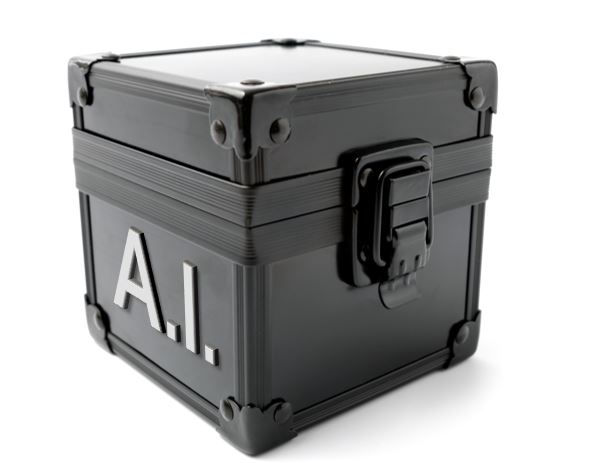
\includegraphics[height=2.5cm]{AI-Box.jpg}} \pause
	\only<7->{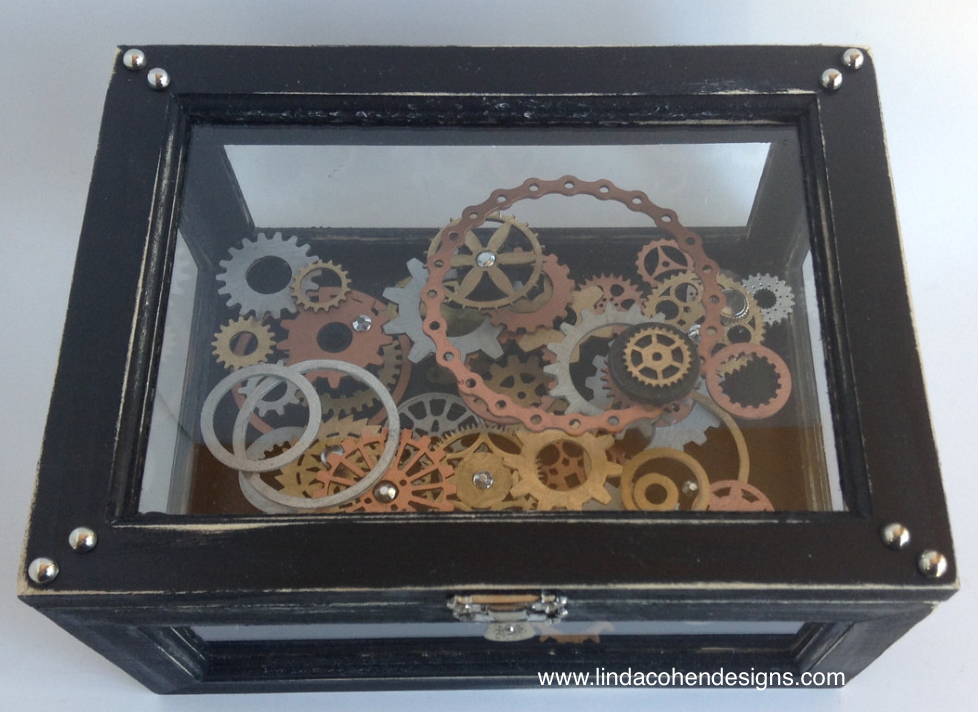
\includegraphics[height=2.5cm]{glass-gear-box.png}}
	\begin{itemize}
		\item e.g. 3-layer neural network
		\item[] $y = \sigma( W^1 \sigma( W^2 \sigma( W^3 X ) ) )$
		\item[] \textbf{what does a particular value of $W^2_{ij}$ mean? \pause }
		\item We can look in the box, but it's hard to interpret.
	\end{itemize}
	
\end{columns}
\vfill
\scriptsize
Image credit: \url{fico.com} ; \url{www.lindacohendesigns.com}
\end{frame}
  
%%% FRAMEBREAK %%%

\begin{frame}{Explanation}
\begin{itemize}[<+->]
	\item Uninterpretable $\rightarrow$ Interpretable
	\item TREPAN (Craven and Shavlik, NIPS 1996)
	\item[] Decision tree
	\item LIME (Ribiero, Singh, and Guestrin, SIGKDD 2016)
	\item[] (locally) Linear model
	\item Anchors (Ribiero, Singh, and Guestrin, AAAI 2018)
	\item[] Conjunctive rules
\end{itemize}

\end{frame}

%%% FRAMEBREAK %%%

\begin{frame}{TREPAN}
\begin{columns}
	\column{0.5\textwidth}
	\begin{itemize}[<+->]
		\item Learns a decision tree from a neural network (NN)
		\item A big challenge to learning decision trees from data is that the amount of relevant samples decreases as the tree gets deeper
		\item TREPAN uses the NN for an oracle to evaluate splits, eliminating this issue
		\item Decision nodes ($n$) to expand are prioritized by
		\item[] $\mathit{reach}( n ) \times (1 - \mathit{fidelity}(n) )$
	\end{itemize}
	\column{6cm}
	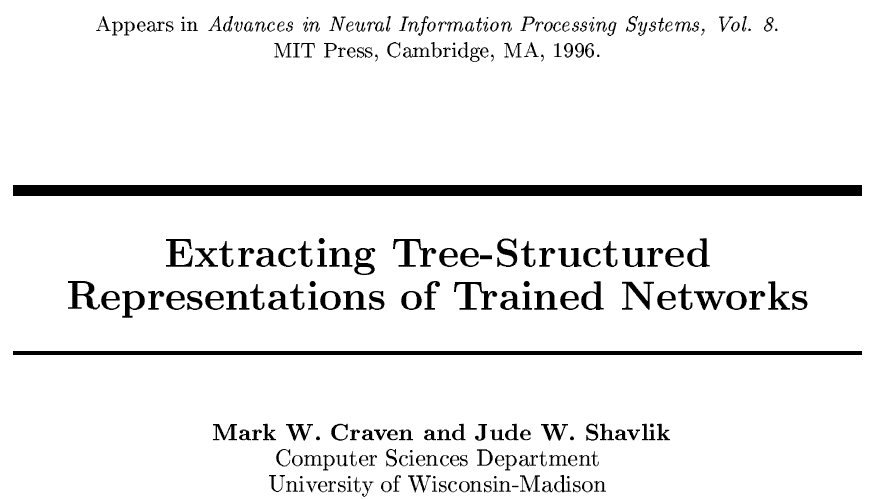
\includegraphics[width=6cm]{trepan-title.png}
	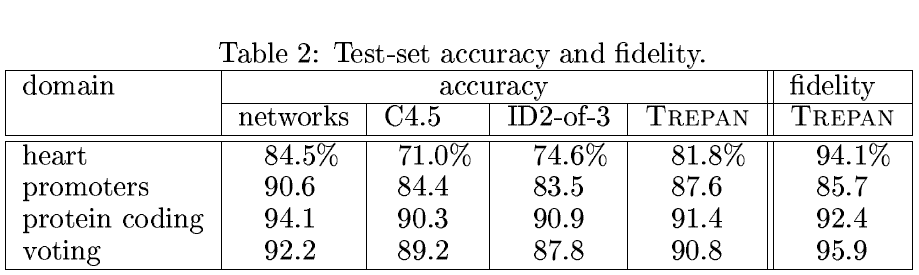
\includegraphics[width=6cm]{trepan-table.png}
\end{columns}
\end{frame}

%%% FRAMEBREAK %%%

\begin{frame}{LIME}
\begin{columns}
	\column{0.47\textwidth} \centering
	
\includegraphics[width=6cm]{LIME-title.png}
	
	{\color{UWRed}
	\[
	\arg \min_g \underbrace{ \mathcal L ( f, g, \pi_x ) }_{\text{fidelity loss around }x} + \underbrace{ \Omega( g ) }_\text{complexity}
	\]}
	
	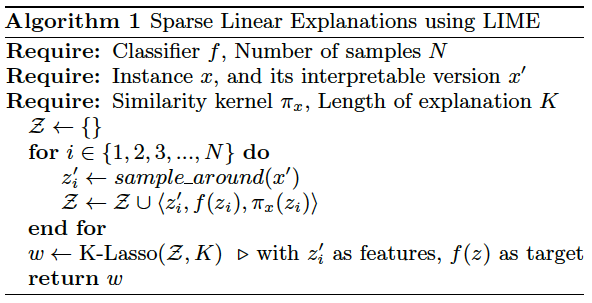
\includegraphics[width=6cm]{LIME-alg.png}
	\column{0.47\textwidth} \centering
	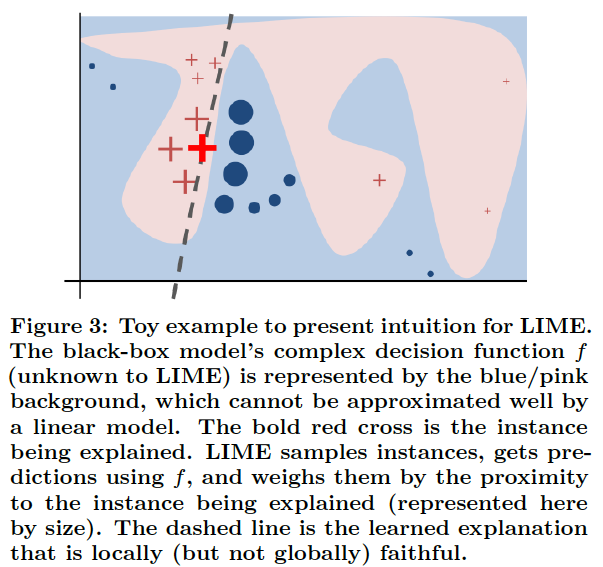
\includegraphics[width=6cm]{LIME-intuition.png}
\end{columns}
\end{frame}

%%% FRAMEBREAK %%%

\begin{frame}{LIME applied to images}
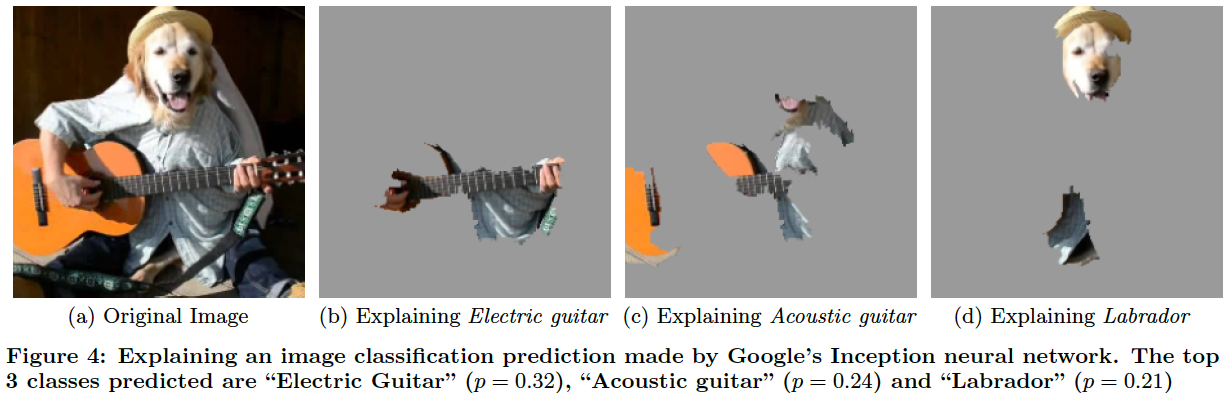
\includegraphics[width=\textwidth]{LIME-image.png}
\end{frame}

%%% FRAMEBREAK %%%

\begin{frame}{Anchors: High-Precision Model-Agnostic Explanations}
\begin{columns}
	\column{0.47\textwidth} \centering
	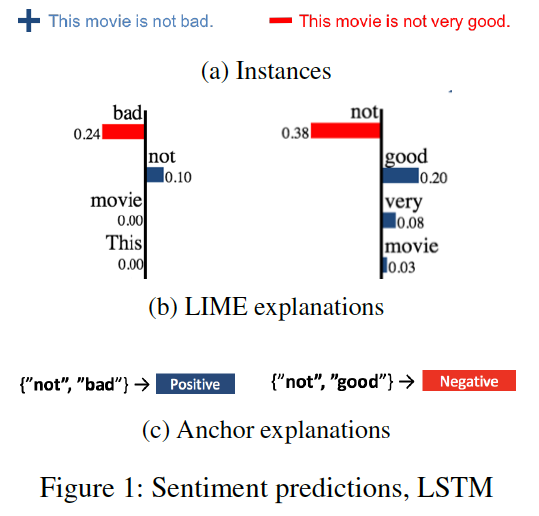
\includegraphics[width=6cm]{anchors-fig1.png} \pause
	\column{0.47\textwidth} \centering
	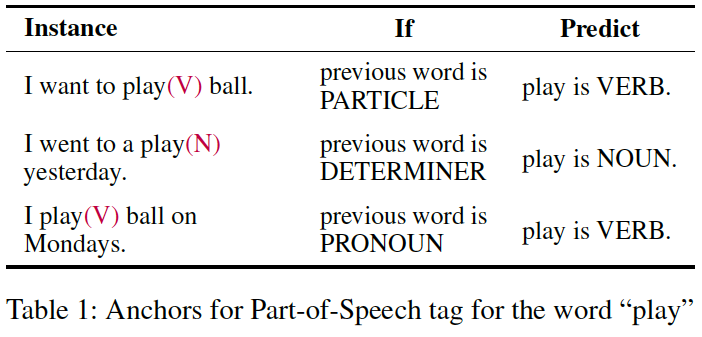
\includegraphics[width=6cm]{anchors-pos.png} \pause
	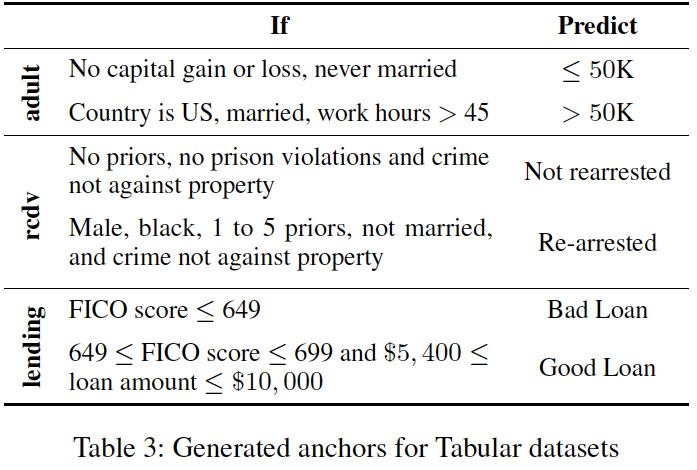
\includegraphics[width=6cm]{anchors-tab.png}	
\end{columns}
\end{frame}

%%% FRAMEBREAK %%%

\begin{frame}{Anchors: formal definition}

\begin{itemize}
	\item An anchor is a rule, formally expressed as a function $A : X \rightarrow \{0,1\}$ \pause
	\item Given a black-box model $f : X \rightarrow Y$
	\begin{itemize}
		\item $X$ is the space of instances
		\item $Y$ is the space of model outputs
	\end{itemize} \pause
	\item $A$  is an anchor iff
	\item[] $\underbrace{\mathbb{E}_{\mathcal D (z | A)} \left[ \mathbf{1}_{f(x)=f(z)} \right] }_{\mathrm{Prec}(A)} \geq \tau$ when $A(x) = 1$
\end{itemize}  \pause
  That is, $A$ is a rule that holds for our sample $x$ and, for any $z$ in the data distribution $\mathcal D$ for which $A$ holds, the output is (probably) the same as for $x$. \pause
  
  To avoid computing the precision directly (intractable) a probabilistic criterion for an anchor is used:
  \[
  P( \mathrm{prec}(A) \geq \tau ) \geq 1 - \delta
  \]
  Since multiple rules can satisfy the criterion, the one with maximum coverage is picked:
  \[
  \max_{A \text{ s.t. } P(\mathrm{prec}(A) \geq \tau ) \geq 1 - \delta} \underbrace{ \mathbb E_{\mathcal D (z) } \left[ A(z) \right] }_{\mathrm{cov}(A)}
  \]
\end{frame}

\begin{frame}{Searching for anchors}
\begin{columns}
	\column{0.47\textwidth}
	\begin{itemize}
		\item The authors present a greedy search for anchors
		\begin{itemize}
			\item does not explicitly maximize coverage
			\item but shorter rules are found first, and shorter rules tend to have higher coverage
		\end{itemize}
		\item Next, they present a beam search that works on similar principles
		\begin{itemize}
			\item does explicitly maximize coverage
		\end{itemize}
	\end{itemize}
	% TODO: KL-LUCB (look up? briefly describe? Kaufmann and Kalyanakrishnan 2013)
	
	\column{0.47\textwidth}
	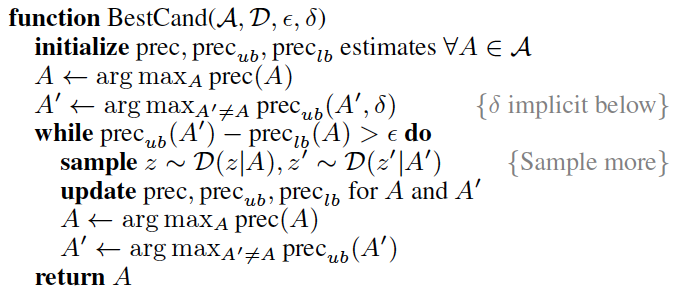
\includegraphics[width=6cm]{anchors-alg.png}
\end{columns}
\end{frame}

\begin{frame}{Anchors: simulated users} \centering
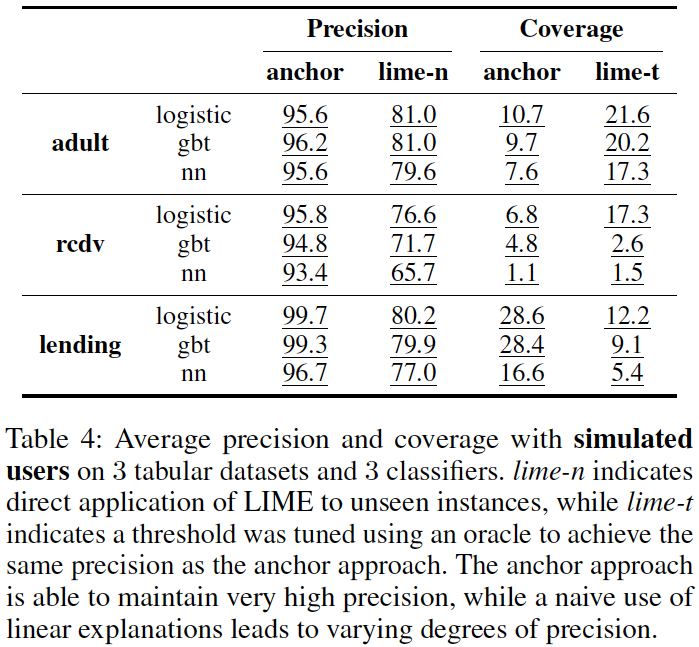
\includegraphics[width=6cm]{anchors-simusers.png}
\end{frame}
\begin{frame}{Anchors: user study} \centering
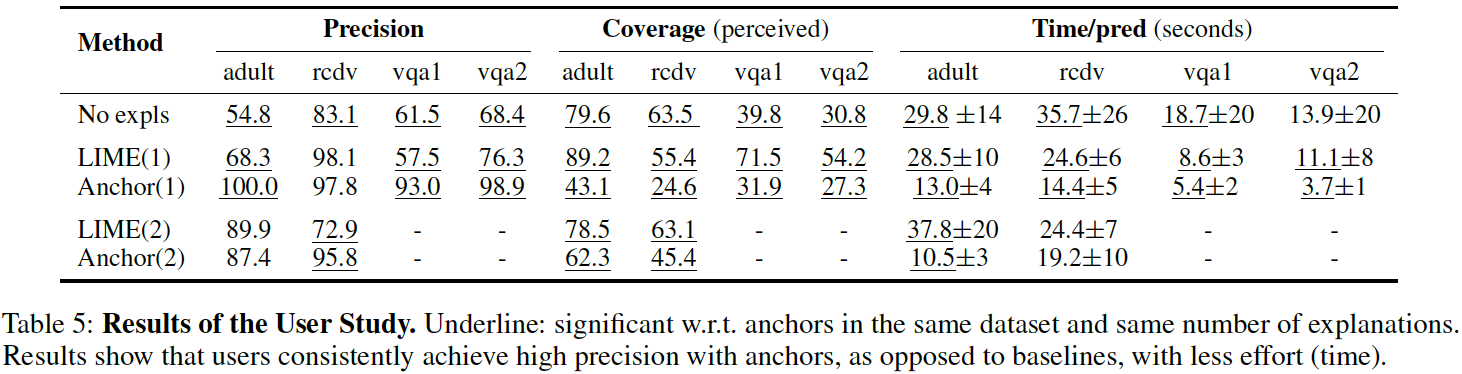
\includegraphics[width=\textwidth]{anchors-userstudy.png}
\end{frame}

%%% FRAMEBREAK %%%

\begin{frame}{Anchors: reflection}
\begin{itemize}
	\item The approach is general: can be applied to any model targeting a variety of tasks, but
	\item Some engineering is involved in:
	\begin{itemize}
		\item designing the perturbation distribution $\mathcal D$
		\item defining what the "atoms" in the anchor rules are
		\item deciding how to display anchors to the user
	\end{itemize}
	\item Various limitations pointed out by authors
\end{itemize}
\end{frame}

\end{document}